
\documentclass[xetex,professionalfont]{beamer}

\usepackage{amsmath}

\usepackage{mathtools}

\usepackage{amssymb}

\usepackage{xspace}

\usepackage{booktabs}


\usepackage{fontspec}
\setmonofont[Scale=0.7]{Droid Sans Mono} %

\usepackage[caption=false]{subfig}
\captionsetup{belowskip=0pt,aboveskip=0pt}

\usepackage{csquotes}

\usepackage{copyrightbox}

\usepackage[english]{babel}


\usepackage{tikz}

\usepackage{pgfplots}

\usetikzlibrary{backgrounds,arrows,automata}

\definecolor{xblue}{RGB}{210,224,255}
\definecolor{xyellow}{RGB}{255,255,205}
\definecolor{xred}{RGB}{255,205,205}
\definecolor{xgreen}{RGB}{205,255,205}


\hypersetup{pdftitle={DLVC Lecture 9},pdfsubject={},pdfauthor={Christopher Pramerdorfer},colorlinks,urlcolor=tuwcvl_cvl_blue,linkcolor=tuwcvl_textlight,citecolor=tuwcvl_textlight}

\makeatletter\renewcommand{\CRB@setcopyrightfont}{\tiny\color{lightgray}}

\let\oldemph\emph
\renewcommand\emph[1]{\textcolor{tuwcvl_cvl_blue}{#1}}

\usefonttheme[onlymath]{serif}

\usetheme{dlvc}


\definecolor{dred}{rgb}{0.85,0,0.1}
\definecolor{dgreen}{rgb}{0,0.85,0.1}
\definecolor{dblue}{rgb}{0,0.1,0.85}


\newcommand{\ie}{\mbox{i.e.}\xspace} %
\newcommand{\eg}{\mbox{e.g.}\xspace} %

\DeclareMathOperator*{\argmin}{arg\,min}
\DeclareMathOperator*{\argmax}{arg\,max}

\newcommand{\NN}{\mathbb{N}}
\newcommand{\ZZ}{\mathbb{Z}}
\newcommand{\QQ}{\mathbb{Q}}
\newcommand{\RR}{\mathbb{R}}

\renewcommand{\vec}[1]{\ensuremath{\mathbf{#1}}}

\newcommand{\va}{\vec{a}}
\newcommand{\vb}{\vec{b}}
\newcommand{\vc}{\vec{c}}
\newcommand{\ve}{\vec{e}}
\newcommand{\vr}{\vec{r}}
\newcommand{\vs}{\vec{s}}
\newcommand{\vt}{\vec{t}}
\newcommand{\vu}{\vec{u}}
\newcommand{\vv}{\vec{v}}
\newcommand{\vw}{\vec{w}}
\newcommand{\vx}{\vec{x}}
\newcommand{\vy}{\vec{y}}
\newcommand{\vz}{\vec{z}}
\newcommand{\vo}{\vec{o}}
\newcommand{\vm}{\vec{m}}
\newcommand{\vn}{\vec{n}}

\makeatletter
\let\@@magyar@captionfix\relax
\makeatother

\newcommand{\vA}{\vec{A}}
\newcommand{\vW}{\vec{W}}
\newcommand{\vX}{\vec{X}}
\newcommand{\bth}{\boldsymbol{\theta}}
\newcommand{\cD}{\mathcal{D}}
\newcommand{\cG}{\mathcal{G}}
\newcommand{\cB}{\mathcal{B}}

\DeclareMathOperator*{\sgn}{sgn}
\DeclareMathOperator*{\mean}{mean}
\DeclareMathOperator*{\iou}{iou}
\DeclareMathOperator*{\ap}{AP}
\DeclareMathOperator*{\map}{mAP}

\makeatletter
\def\verbatim@font{\linespread{1}\normalfont\ttfamily}
\makeatother


\title{Deep Learning for Visual Computing}
\subtitle{Dense Prediction}
\author{Christopher Pramerdorfer}
\institute{Computer Vision Lab, TU Wien}

\begin{document}


\begin{frame}
	\maketitle
\end{frame}


\begin{frame}
	\frametitle{Topics}

	Dense prediction
	\begin{itemize}
		\item Semantic image segmentation
		\item Keypoint detection
		\item Image restoration
	\end{itemize}

	\bigskip

	Building blocks
	\begin{itemize}
		\item Upsampling layers
		\item U-Nets \& Conditional GANs
	\end{itemize}

\end{frame}


\begin{frame}
	\frametitle{This Week in AI}
	\framesubtitle{Drag Your GAN}

	\begin{center}
		\copyrightbox[b]
		{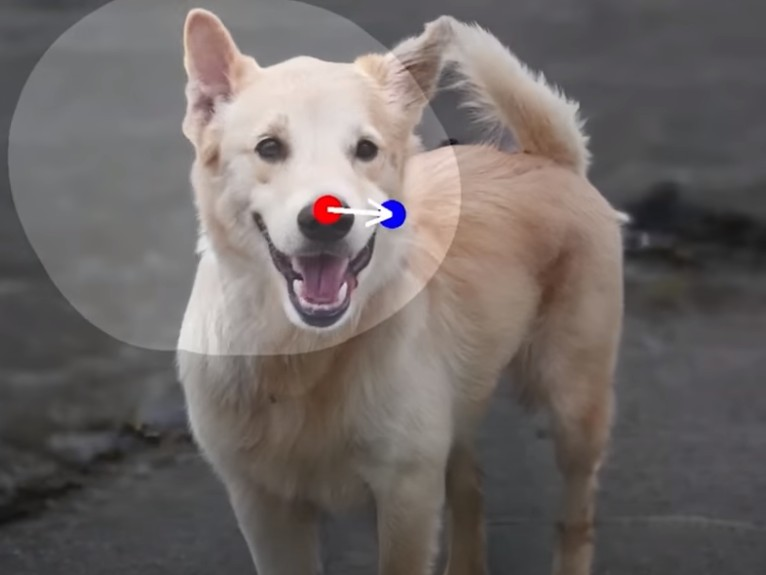
\includegraphics[width=7cm]{images/drag-your-gan.jpg}}
		{\centering Image from \href{https://www.youtube.com/watch?v=BPSv6veX1HA}{youtube}}
	\end{center}

\end{frame}


\begin{frame}
	\frametitle{Dense Prediction}

	We often want to predict something for every input image pixel
	\begin{itemize}
		\item This is called \emph{dense prediction}
		\item How can we achieve that?
	\end{itemize}

	\bigskip

	Obvious solution is to avoid pooling
	\begin{itemize}
		\item We already established this is too slow
		\item Also receptive field increases slowly so missing context %
	\end{itemize}

\end{frame}


\begin{frame}
	\frametitle{Dense Prediction}

	Solution is to use an \emph{encoder-decoder architecture}
	\begin{itemize}
		\item \emph{Encoder} learns high-level features
		\item \emph{Decoder} maps these features back to original size
	\end{itemize}

	\medskip

	\begin{center}
		\copyrightbox[b]
		{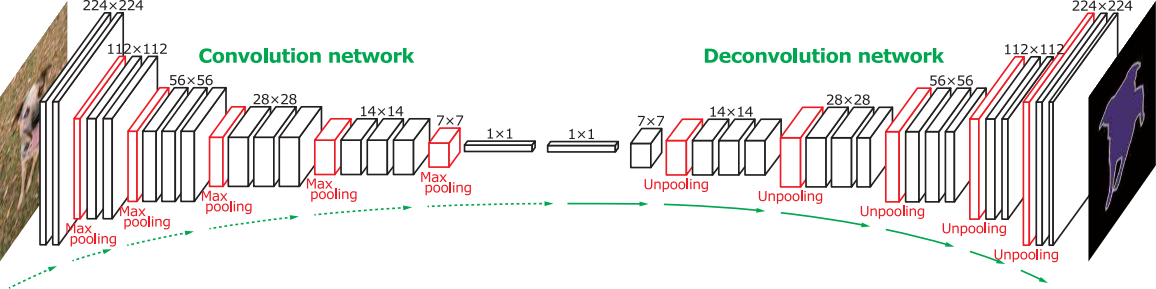
\includegraphics[width=10.5cm]{images/downsample-upsample}} %
		{\centering Image from [1]}
	\end{center}

\end{frame}


\begin{frame}
	\frametitle{Dense Prediction}

	Layer types
	\begin{itemize}
		\item Encoder: conv and pooling layers (e.g. ResNet)
		\item Decoder: conv and \emph{upsampling} layers
	\end{itemize}

	\medskip

	\begin{center}
		\copyrightbox[b]
		{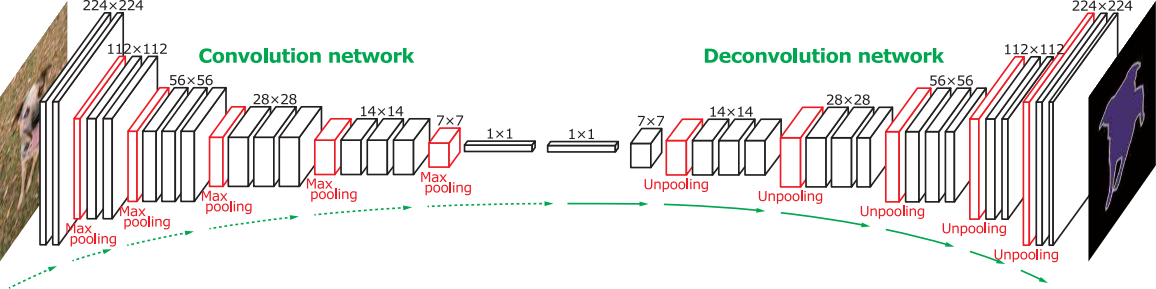
\includegraphics[width=10.5cm]{images/downsample-upsample}} %
		{\centering Image from [1]}
	\end{center}

\end{frame}


\begin{frame}
	\frametitle{Dense Prediction}
	\framesubtitle{Upsampling -- Interpolatuion}

	One way is to utilize standard 2D upsampling techniques
	\begin{itemize}
		\item Nearest neighbor or bilinear interpolation
		\item Independently per channel
	\end{itemize}

	\bigskip

	Fast and simple

	\bigskip

	Usually paired with a conv layer
	\begin{itemize}
		\item To learn useful features / transformations
	\end{itemize}

\end{frame}


\begin{frame}
	\frametitle{Dense Prediction}
	\framesubtitle{Upsampling -- Interpolation}

	Example (\enquote{inverse max-pooling}) %
	\begin{itemize}
		\item Upsampling by factor of 2
		\item Nearest neighbor interpolation
	\end{itemize}

	\medskip

	\[
		\begin{bmatrix}
			1 & 2 \\
			3 & 4
		\end{bmatrix}
		\quad\Longrightarrow\quad
		\begin{bmatrix}
			1 & 1 & 2 & 2 \\
			1 & 1 & 2 & 2 \\
			3 & 3 & 4 & 4 \\
			3 & 3 & 4 & 4
		\end{bmatrix}
	\]

\end{frame}


\begin{frame}
	\frametitle{Dense Prediction}
	\framesubtitle{Upsampling -- Transposed Convolutions}

	\emph{Transposed convolutions} are convolutions with stride $1/s$ %
	\begin{itemize}
		\item Also called \emph{fractionally strided convolutions}
		\item See link below for animations of variants
	\end{itemize}

	\medskip

	\begin{center}
		\copyrightbox[b]
		{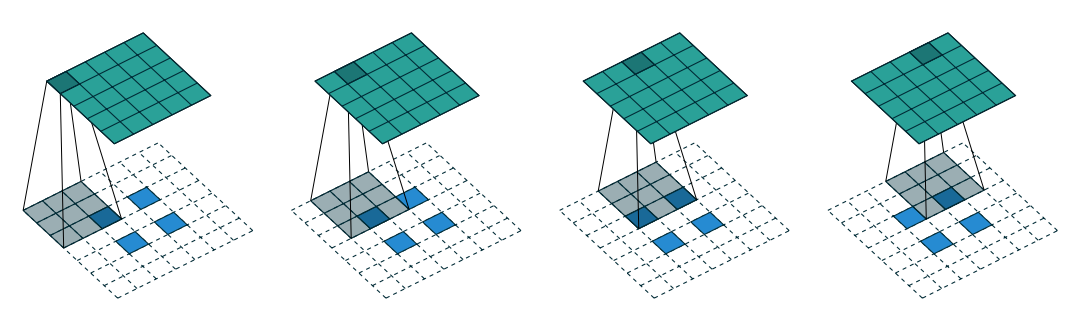
\includegraphics[width=10.5cm]{images/transposed-conv}}
		{\centering Image from \href{https://github.com/vdumoulin/conv\_arithmetic}{github}}
	\end{center}

\end{frame}


\begin{frame}
	\frametitle{Dense Prediction}
	\framesubtitle{Upsampling -- Transposed Convolutions}

	Learnable upsampling
	\begin{itemize}
		\item More powerful than pure interpolation
		\item But often leards to artifacts due to overlapping kernel
	\end{itemize}

	\medskip

	\begin{center}
		\copyrightbox[b]
		{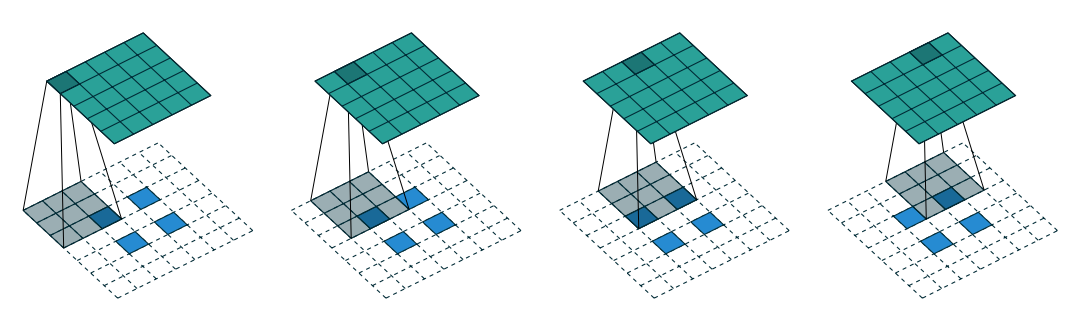
\includegraphics[width=10.5cm]{images/transposed-conv}}
		{\centering Image from \href{https://github.com/vdumoulin/conv\_arithmetic}{github}}
	\end{center}

\end{frame}


\begin{frame}
	\frametitle{Dense Prediction}
	\framesubtitle{Upsampling -- Subpixel Convolutions}

	\emph{Subpixel convolutions} are most recent upsampling method
	\begin{itemize}
		\item Usually outperforms other methods covered
		\item Also called \emph{pixel shuffle}
	\end{itemize}

	\bigskip

	Operation
	\begin{itemize}
		\item Given input of size $(C\cdot r^2)\times H\times W$ %
		\item Rearange (shuffle) to $C\times rH\times rW$
		\item Then do a stride $1$ convolution
	\end{itemize}

\end{frame}


\begin{frame}
	\frametitle{Dense Prediction}
	\framesubtitle{Upsampling -- Subpixel Convolutions}

	Example with $r=3$ and $9\times7\times7$ input


	\bigskip

	\begin{center}
		\copyrightbox[b]
		{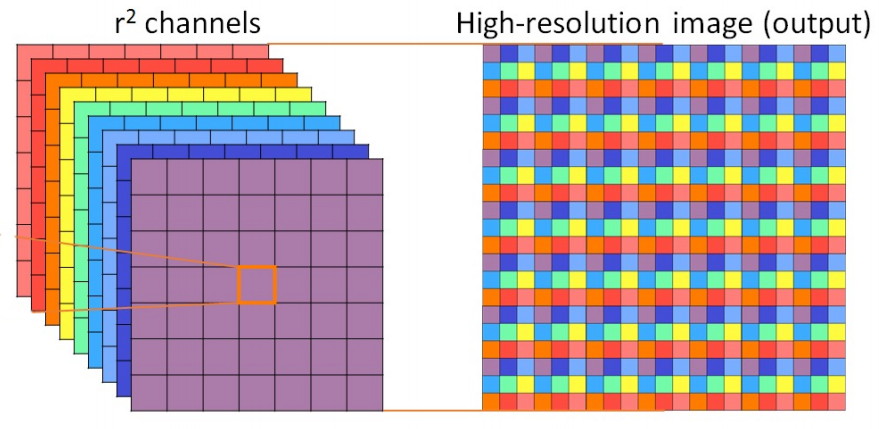
\includegraphics[width=8cm]{images/pixel-shuffle}}
		{\centering Image from [4]}
	\end{center}

\end{frame}


\begin{frame}
	\frametitle{Dense Prediction}

	We can train such networks like we did before
	\begin{itemize}
		\item Gradient descent and backpropagation
		\item Just define a suitable loss depending on task
	\end{itemize}

	\bigskip

	\begin{center}
		\copyrightbox[b]
		{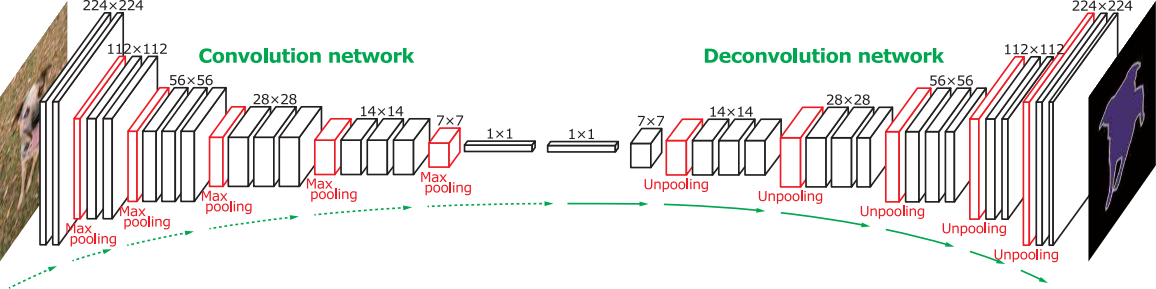
\includegraphics[width=10.5cm]{images/downsample-upsample}}
		{\centering Image from [1]}
	\end{center}

\end{frame}


\begin{frame}
	\frametitle{Dense Prediction}

	However this would probably not work very well because
	\begin{itemize}
		\item The network has no idea how objects look like
		\item Spatial information is lost due to excessive downsampling
	\end{itemize}

	\bigskip

	\begin{center}
		\copyrightbox[b]
		{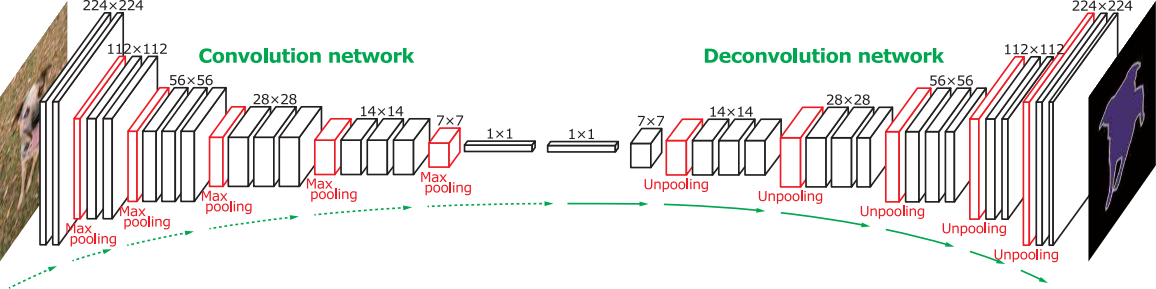
\includegraphics[width=10.5cm]{images/downsample-upsample}}
		{\centering Image from [1]}
	\end{center}

\end{frame}


\begin{frame}
	\frametitle{Dense Prediction}

	To address this we
	\begin{itemize}
		\item Pre-train the encoder (e.g.~ImageNet classification)
		\item Use skip-connections across the two parts
	\end{itemize}

	\bigskip

	\begin{center}
		\copyrightbox[b]
		{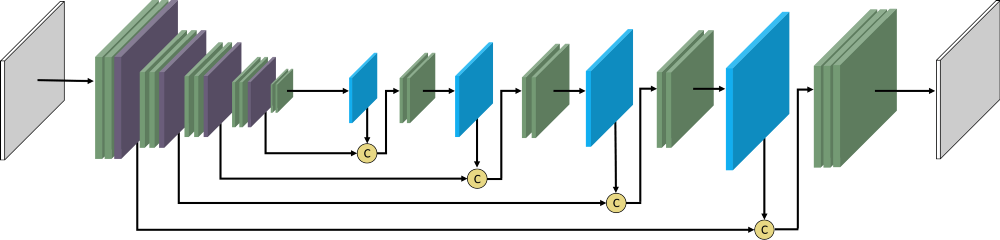
\includegraphics[width=10.5cm]{images/unet}}
		{\centering Image from medium.com}
	\end{center}

\end{frame}


\begin{frame}
	\frametitle{Dense Prediction}
	\framesubtitle{U-Nets}

	A popular method for defining these connections is \emph{U-Net} [2]
	\begin{itemize}
		\item Skip from before every downsampling layer
		\item To after every corresponding upsampling layer
		\item \emph{Concatenate} (not sum) signals
	\end{itemize}

	\bigskip

	\begin{center}
		\copyrightbox[b]
		{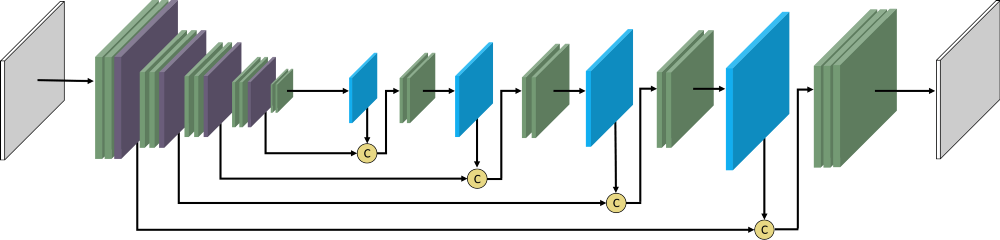
\includegraphics[width=10.5cm]{images/unet}}
		{\centering Image from medium.com}
	\end{center}

\end{frame}


\begin{frame}
	\frametitle{Dense Prediction}
	\framesubtitle{U-Nets}

	Skip-connections forward high-resolution data
	\begin{itemize}
		\item Makes spatial information available to decoder
		\item Signals are concatenated due to different nature %
	\end{itemize}

	\bigskip

	\begin{center}
		\copyrightbox[b]
		{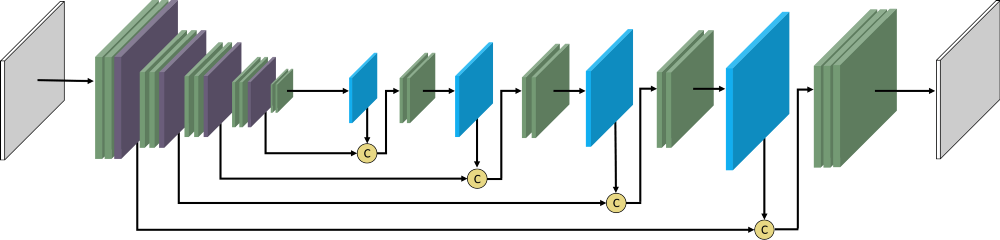
\includegraphics[width=10.5cm]{images/unet}}
		{\centering Image from medium.com}
	\end{center}

\end{frame}


\begin{frame}
	\frametitle{Dense Prediction}
	\framesubtitle{U-Nets}

	Modern U-Nets often use
	\begin{itemize}
		\item A ResNet for downsampling
		\item Subpixel convolutions for upsampling
	\end{itemize}

	\bigskip

	\begin{center}
		\copyrightbox[b]
		{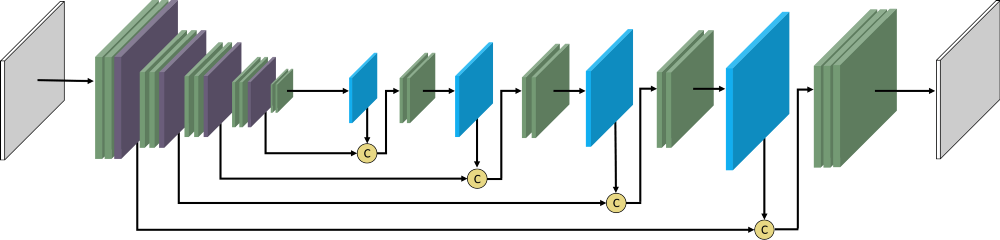
\includegraphics[width=10.5cm]{images/unet}}
		{\centering Image from medium.com}
	\end{center}

\end{frame}


\begin{frame}
	\frametitle{Dense Prediction}
	\framesubtitle{Applications}

	We now have all we need to solve various tasks
	\begin{itemize}
		\item Simply choose $C$ of output accordingly
		\item And use a suitable loss function
		\item Always pre-train the encoder
	\end{itemize}

	\bigskip
	We will cover three popular applications

\end{frame}


{
\setbeamertemplate{footline}{}
\begin{frame}

	\begin{tikzpicture}[remember picture,overlay]
		\fill[white] (current page.north west) rectangle (current page.south east);
	\end{tikzpicture}

	\begin{center}
		\textcolor[rgb]{0.9,0.9,0.9}{blank page}
	\end{center}

\end{frame}
}


\begin{frame}
	\frametitle{Semantic Image Segmentation}

	Task definition
	\begin{itemize}
		\item Given $T$ classes
		\item Assign a class label to each image pixel
	\end{itemize}

	\medskip

	\begin{center}
		\copyrightbox[b]
		{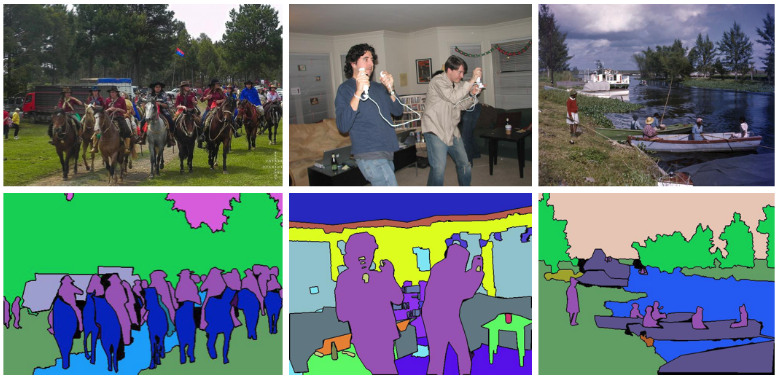
\includegraphics[width=8cm]{images/coco.jpg}}
		{\centering Image from \href{http://cocodataset.org}{cocodataset.org}}
	\end{center}

\end{frame}


\begin{frame}
	\frametitle{Semantic Image Segmentation}

	Implementation
	\begin{itemize}
		\item Configure last layer to output $T$ channels
		\item Use cross-entropy loss $L_p(\bth)$ for every pixel $p$
		\item Minimize $L(\bth)=\sum_pL_p(\bth)$ %
	\end{itemize}

\end{frame}


\begin{frame}
	\frametitle{Keypoint Detection}

	\emph{Keypoint detection} task definition
	\begin{itemize}
		\item Given $K$ \emph{keypoints}
		\item Locate each keypoint in image (multiple times)
	\end{itemize}

	\bigskip
	A popular application is (sparse) \emph{human pose estimation}
	\begin{itemize}
		\item Keypoints for hands, feet, shoulders etc.
	\end{itemize}

\end{frame}


\begin{frame}
	\frametitle{Keypoint Detection}

	Implementation
	\begin{itemize}
		\item Configure last layer to output $K$ channels
		\item Each channel encodes keypoint confidences (\emph{confidence map})
		\item Use e.g. L2 loss $L_c(\bth)$ (\emph{MSE loss}) for every channel $c$ %
		\item Minimize $L(\bth)=\sum_cL_c(\bth)$ %
	\end{itemize}

	\bigskip
	Supporting multiple instances requires keypoint matching
	\begin{itemize}
		\item Can be done in post-processing step
	\end{itemize}

\end{frame}


\begin{frame}
	\frametitle{Keypoint Detection}

	Note that dense prediction is not mandatory
	\begin{itemize}
		\item Could simply regress keypoint coordinates
	\end{itemize}

	\bigskip
	But dense prediction is more flexible \& powerful
	\begin{itemize}
		\item Confidences facilitate downstream tasks
		\item Can predict additional dense data (e.g.~part affinity fields)
	\end{itemize}

	\medskip
	\begin{center}
		\copyrightbox[b]
		{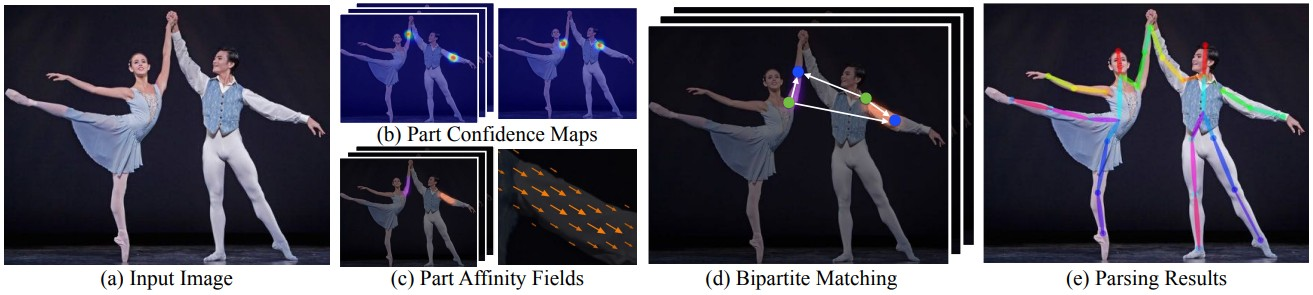
\includegraphics[width=10cm]{images/openpose-method.jpg}}
		{\centering Image from [3]}
	\end{center}

\end{frame}


\begin{frame}
	\frametitle{Keypoint Detection}

	Human pose estimation with OpenPose [3]
	\bigskip

	\begin{center}
		\copyrightbox[b]
		{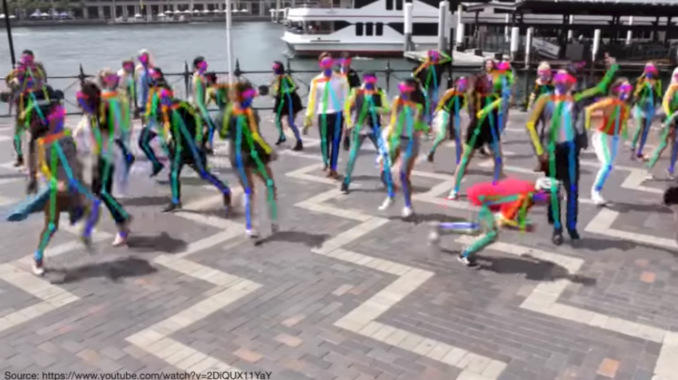
\includegraphics[width=7cm]{images/pose}}
		{\centering\href{https://www.youtube.com/watch?v=pW6nZXeWlGM}{link}}
	\end{center}

\end{frame}


\begin{frame}
	\frametitle{Image Restoration}

	\emph{Image restoration} aims to improve image quality

	\bigskip

	Common tasks
	\begin{itemize}
		\item Remove overlays and compression artifacts
		\item Sharpen or upscale
	\end{itemize}

	\medskip

	\begin{center}
		\copyrightbox[b]
		{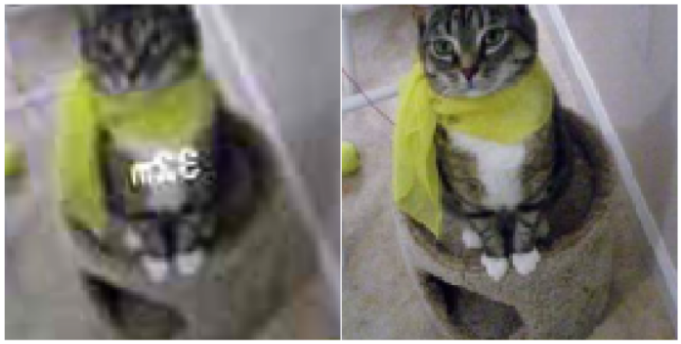
\includegraphics[width=5.5cm]{images/image-restoration}}
		{\centering Image from medium.com}
	\end{center}

\end{frame}


\begin{frame}
	\frametitle{Image Restoration}

	Implementation
	\begin{itemize}
		\item Configure last layer to output $C_0$ channels (usually $C_0=3$)
		\item Train on pairs of low-quality and high-quality images
		\item Use L2 loss $L_p(\bth)$ for every pixel $p$
		\item Minimize $L(\bth)=\sum_pL_p(\bth)$
	\end{itemize}

\end{frame}


\begin{frame}
	\frametitle{Image Restoration}

	Generating large datasets is comparatively easy %
	\begin{itemize}
		\item Take high-quality images
		\item Degrade them automatically depending on task (e.g.~blur) %
	\end{itemize}

	\bigskip

	\begin{center}
		\copyrightbox[b]
		{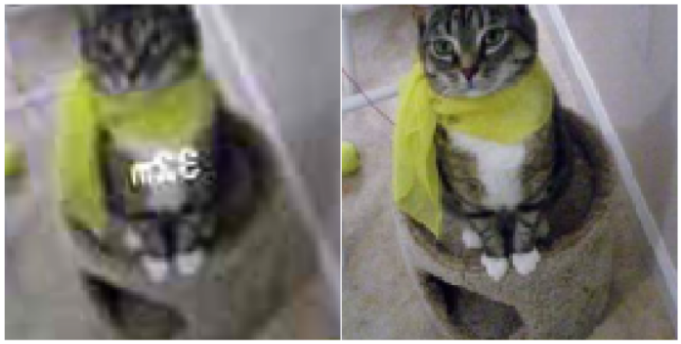
\includegraphics[width=5.5cm]{images/image-restoration}}
		{\centering Image from medium.com}
	\end{center}

\end{frame}


\begin{frame}
	\frametitle{Image Restoration}

	The resulting network would probably be
	\begin{itemize}
		\item Good at removing text and compression artifacts
		\item Not so good at sharpening the image
	\end{itemize}

	\medskip

	\begin{center}
		\copyrightbox[b]
		{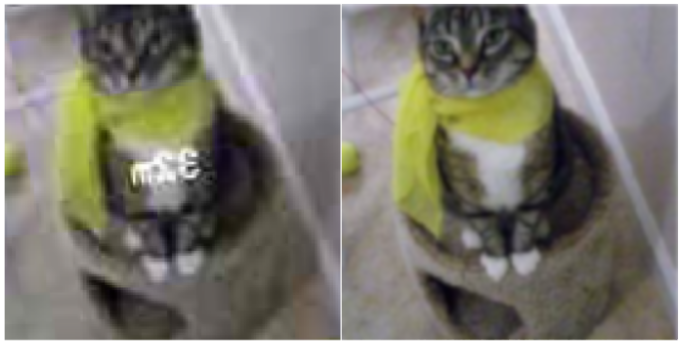
\includegraphics[width=5.5cm]{images/image-restoration-blur}}
		{\centering Image from medium.com}
	\end{center}

\end{frame}


\begin{frame}
	\frametitle{Image Restoration}

	Because L2 loss does not capture sharpness well
	\begin{itemize}
		\item Blurring has little effect on most pixel values
		\item Per-pixel losses cannot capture overall sharpness
	\end{itemize}

	\medskip

	\begin{center}
		\copyrightbox[b]
		{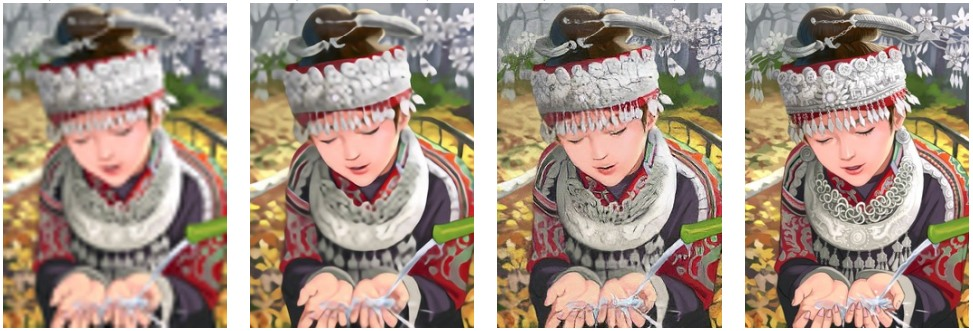
\includegraphics[width=10cm]{images/deep-upscale}}
		{\centering Image from [4]}
	\end{center}

\end{frame}


\begin{frame}
	\frametitle{Image Restoration}

	Unclear how to define a good loss for sharpness
	\begin{itemize}
		\item Maybe we can \enquote{learn} it?
	\end{itemize}

	\bigskip
	To do so we use an \emph{adversarial loss}
	\begin{itemize}
		\item Loss function is a binary classifier $\cD$ (\emph{discriminator} or \emph{critic})
		\item That answers \enquote{is the given image real or fake?} %
	\end{itemize}

	\bigskip
	In our context of image restoration
	\begin{itemize}
		\item \enquote{real} means an original high-quality image
		\item \enquote{fake} means one processed by the network
	\end{itemize}
\end{frame}


\begin{frame}
	\frametitle{Image Restoration}
	\framesubtitle{GANs}

	This is a \emph{Conditional Generative Adversarial Network} (\emph{GAN})
	\begin{itemize}
		\item \emph{Generator} $\cG$ (our encoder-decoder) learns to fool the critic
		\item Critic learns not to be fooled
	\end{itemize}

	\smallskip
	\begin{center}
		\copyrightbox[b]
		{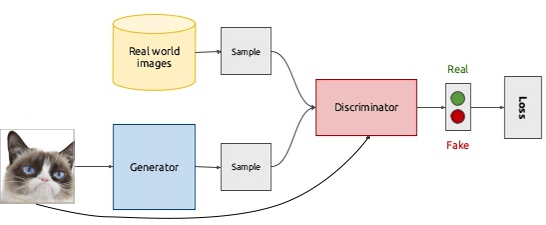
\includegraphics[width=9cm]{images/igan}}
		{\centering Image from sigmoidal.io}
	\end{center}
\end{frame}


\begin{frame}
	\frametitle{Image Restoration}
	\framesubtitle{GANs}

	If $\cG$ can reliably fool $\cD$
	\begin{itemize}
		\item Processed images look just like high-quality ones
		\item And thus must be high-quality themselves
	\end{itemize}

	\smallskip
	\begin{center}
		\copyrightbox[b]
		{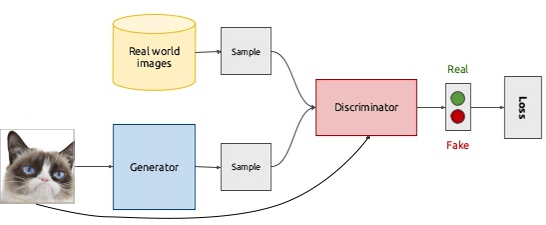
\includegraphics[width=9cm]{images/igan}}
		{\centering Image from sigmoidal.io}
	\end{center}
\end{frame}


\begin{frame}
	\frametitle{Image Restoration}
	\framesubtitle{GANs}

	$\cG$ and $\cD$ form a single network during training
	\begin{itemize}
		\item Gradients flow from $\cD$ to $\cG$
		\item So $\cG$ learns via (cross-entropy) loss on $\cD$
	\end{itemize}

	\smallskip
	\begin{center}
		\copyrightbox[b]
		{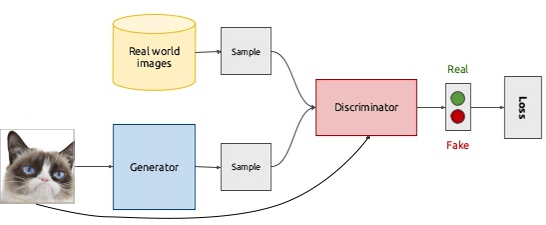
\includegraphics[width=9cm]{images/igan}}
		{\centering Image from sigmoidal.io}
	\end{center}
\end{frame}


\begin{frame}
	\frametitle{Image Restoration}
	\framesubtitle{GANs}

	Training is an iterative process
	\begin{itemize}
		\item Train $\cD$ (but not $\cG$) on real and fake images
		\item Train $\cG$ (but not $\cD$) on fake images
		\item Repeat
	\end{itemize}

	\bigskip

	Loss usually does not converge
	\begin{itemize}
		\item Look at generated images during training
		\item Accuracy of $\cD$ should eventually be $\approx0.5$
	\end{itemize}

\end{frame}


\begin{frame}[fragile]
	\frametitle{Image Restoration}
	\framesubtitle{GANs}

	Typical training loop (many variants exist)
	\begin{itemize}
		\item $k$ is a hyperparameter (often $k=1$ works fine)
	\end{itemize}

	\medskip

	\begin{verbatim}
while not done:
  for k iterations:
    sample half of mini-batch from dataset (class real)
    sample half of mini-batch from G (class fake)
    train D on mini-batch (but not G)
  
  sample mini-batch from G (class real (!))
  train G trough D on mini-batch (but not D itself)
\end{verbatim}


\end{frame}

\begin{frame}
	\frametitle{GANs}

	GANs are a flexible framework with many applications
	\begin{itemize}
		\item More in next lecture
	\end{itemize}

	\bigskip
	Make sure to pre-train both $\cG$ and $\cD$ (if possible)
	\begin{itemize}
		\item Training GANs from scratch is a pain
	\end{itemize}
\end{frame}


\renewcommand\emph[1]{\oldemph{#1}}

\begin{frame}
	\frametitle{Bibliography}

	[1] Noh et al.~\href{https://arxiv.org/abs/1505.04366}{Deconvolution Networks}.~2015 \\\medskip
	[2] Ronneberger et al.~\href{https://arxiv.org/abs/1505.04597}{U-Net}.~2015 \\\medskip
	[3] Cao et al.~\href{https://arxiv.org/abs/1812.08008}{OpenPose}.~2018 \\\medskip
	[4] Shi et al.~\href{https://arxiv.org/abs/1609.05158}{Subpixel Convolutions}.~2016

\end{frame}


\end{document}
